\documentclass[pdftex,12pt,a4paper]{report}
\usepackage[portuges]{babel}
\usepackage[utf8]{inputenc}
\usepackage{t1enc}
\usepackage{fancyhdr}
\usepackage{times}
\usepackage{alltt}
\usepackage{graphicx}% para poder utilizar imagens
\usepackage{fancyvrb}% para Verbatim
\usepackage{url}

\usepackage{multirow}

%-----------------------------------------------------------------------------------
%-- Definições: preencher com os valores específicos de 
%--                      cada proposta
%-----------------------------------------------------------------------------------
\newcommand{\titulo}{DRAFTER+}
\newcommand{\subtitulo}{Requisitos de uma plataforma que auxilie na produção de atos normativos}
\newcommand{\data}{24 de Abril de 2024}
\newcommand{\dataansi}{20240424}
\newcommand{\destinatario}{Direção Geral de Política da Justiça}
\newcommand{\destsigla}{DGPJ}
\newcommand{\proponente}{Universidade do Minho}
\newcommand{\keep}{\textsc{UM}}

%-------------------------------------------------------------------------
%--  Arranjo gráfico das páginas e da mancha de texto
%-------------------------------------------------------------------------
\usepackage[twoside,verbose,body={16cm,24cm},
			left=30mm,top=20mm]{geometry}
			
\pagestyle{fancy}

\fancyfoot{}% clear all defaults for footers
\fancyhead{}% clear all defaults for headers
\fancyfoot[RO]{\small \copyright \ \proponente \ \ \thepage}
\fancyfoot[LE]{\small \thepage\ \ \copyright \ \proponente}

\fancyhead[RO]{\small \leftmark} 
\fancyhead[LE]{\small \titulo}
\renewcommand{\headrulewidth}{0.3pt}% Espessura da linha que separa o header

\fancypagestyle{plain}{%
\fancyhf{} % limpa todos os headers e footers deste estilo
\fancyfoot[RO]{\small \copyright \ \proponente \ \ \thepage}
\renewcommand{\headrulewidth}{0pt}
}

%-------------------------------------------------------------------------
%--  Cabeçalhos dos capítulos
%-------------------------------------------------------------------------
\usepackage[Lenny]{fncychap}
\makeatletter 
  \renewcommand{\DOCH}{%
    \settoheight{\myhi}{\CTV\FmTi{Test}}
    \setlength{\py}{\baselineskip}
    \addtolength{\py}{\RW}
    \addtolength{\py}{\myhi}
    \setlength{\pyy}{\py}
    \addtolength{\pyy}{-1\RW}
     
    \raggedright
    \CNoV\thechapter
    \hskip 3pt\mghrulefill{\RW}\rule[-1\pyy]{2\RW}{\py}\par\nobreak}

  \renewcommand{\DOTI}[1]{%
    \addtolength{\pyy}{-4pt}
    \settoheight{\myhi}{\CTV\FmTi{#1}}
    \addtolength{\myhi}{\py}
    \addtolength{\myhi}{-1\RW}
    \vskip -1\pyy
    \rule{2\RW}{\myhi}\mghrulefill{\RW}\hskip 2pt
    \raggedleft\CTV\FmTi{#1}\par\nobreak
    \vskip 50\p@}
\makeatother

\parindent=0pt

\setlength{\parskip}{.5\baselineskip}% Distância entre paragráfos

%-------------------------------------------------------------------------
%--  Espaço entre linhas
%-------------------------------------------------------------------------
\usepackage{setspace}
\onehalfspacing
%\doublespacing

%-------------------------------------------------------------------------
%--  As minhas macros
%-------------------------------------------------------------------------
\newcommand{\figura}[4]{% label, ficheiro, titulo, opções
  \begin{figure}[htp]%
  \begin{center}%
  \includegraphics[#4]{#2}%
  \end{center}%
  \textbf{\caption{\label{#1} #3}}%
  \end{figure}}

%-----------------------------------------------------------------------------------
%-- Início
 
\newcommand{\HRule}{\rule{\linewidth}{0.5mm}}
 
\begin{document}
 
\begin{titlepage}
 
\begin{tabular*}{\textwidth}%
    [b] {@{\extracolsep{0.5cm}}lr}

\begin{minipage}{0.6\textwidth}
\begin{flushleft}
% Upper part of the page
\vspace{3cm}

\includegraphics{./eeng.png}\\
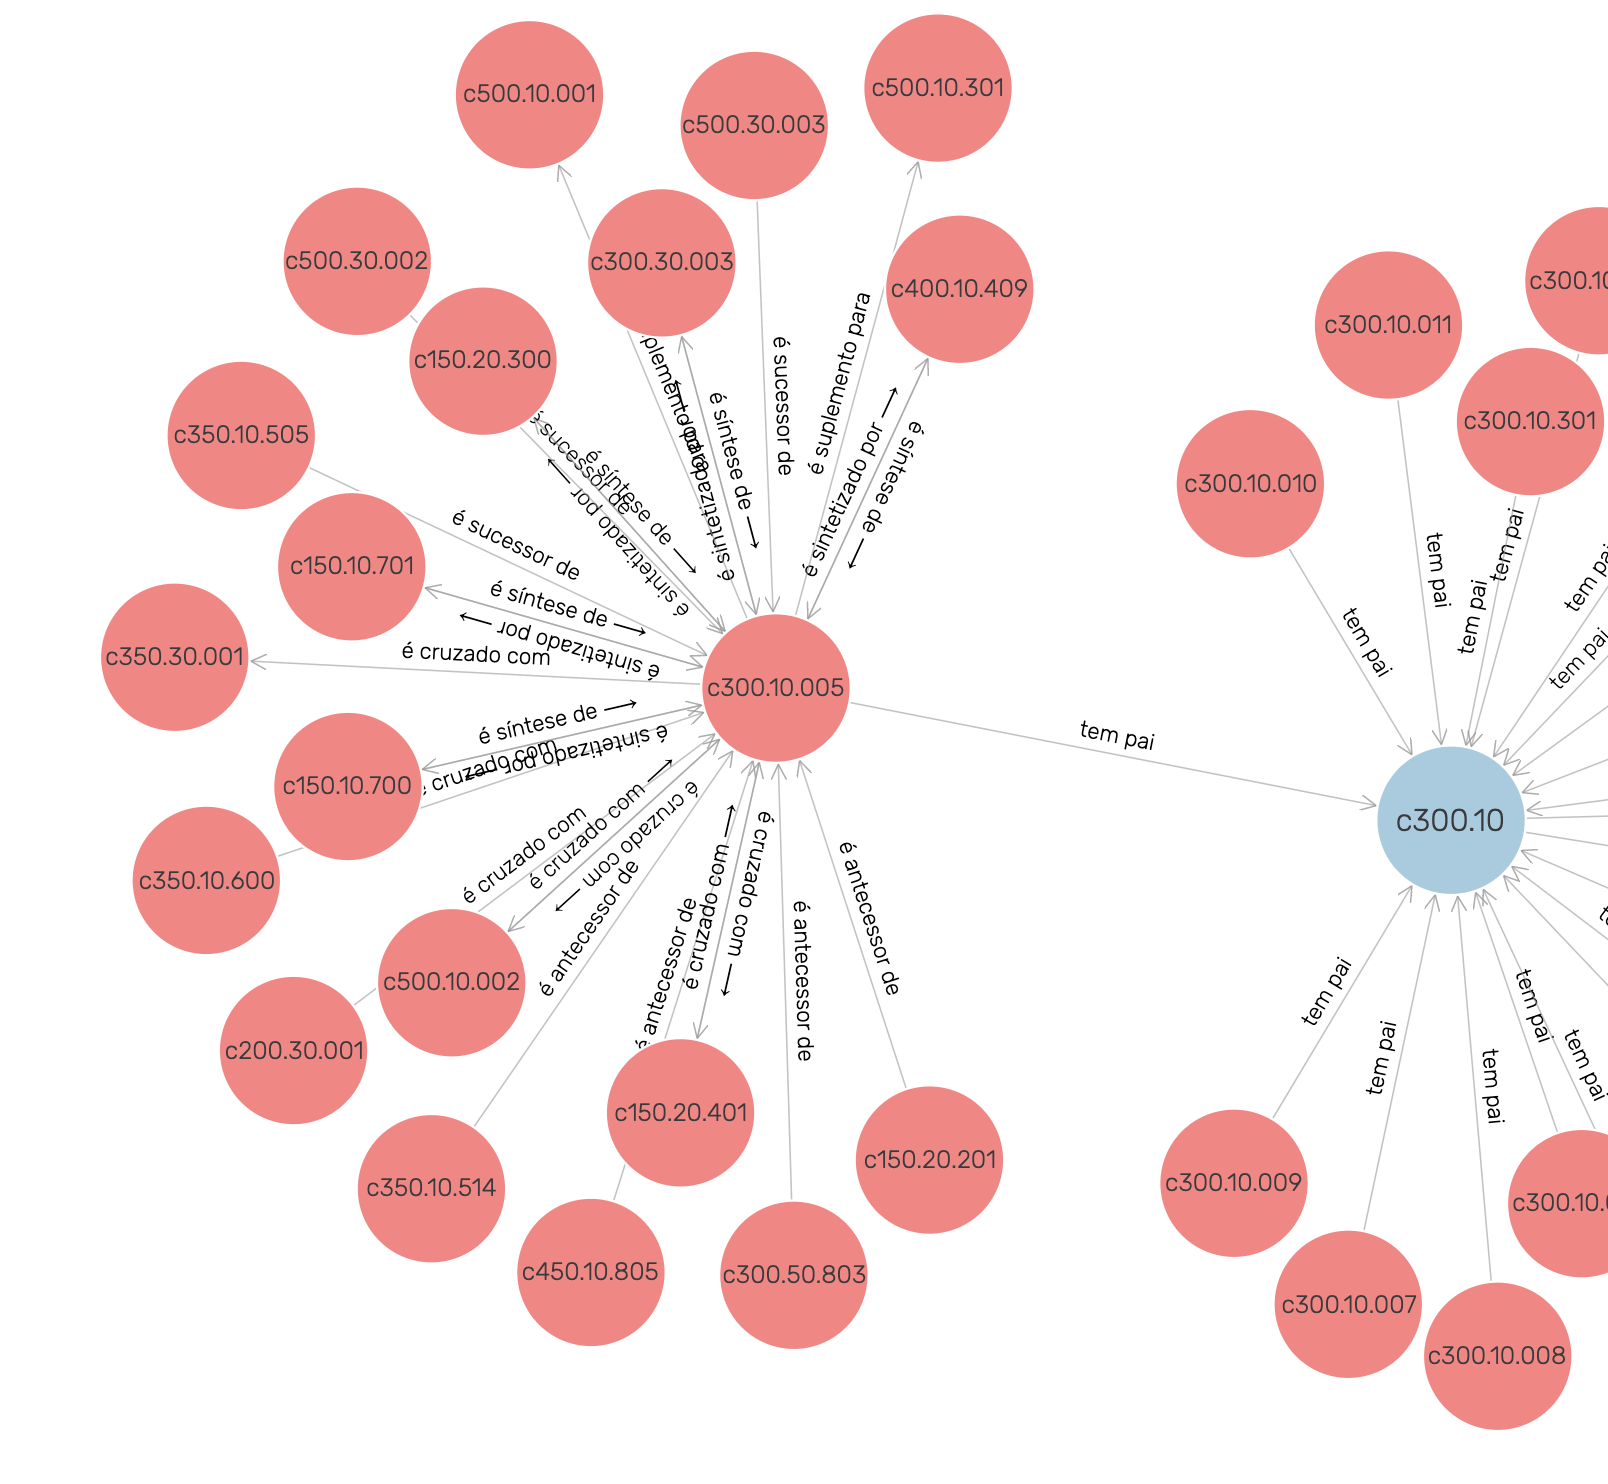
\includegraphics[width=5cm]{./onto.png}\\
\end{flushleft}
\end{minipage}

&

\begin{minipage}{0.4\textwidth}

\vspace{2cm}

 \begin{flushleft}
 
\textsc{\LARGE 
\textbf{\titulo}
}\\[1.5cm]
 
\large \subtitulo
 
\vspace{6cm}

\data
 
\end{flushleft}
\end{minipage}

\\
\end{tabular*}
 
\end{titlepage}


\begin{titlepage}
 
\begin{tabular*}{\textwidth}%
    [b] {@{\extracolsep{0.5cm}}lr}

\begin{minipage}{0.6\textwidth}
\begin{flushleft}
% Upper part of the page
\vspace{3cm}

\includegraphics{./eeng.png}\\
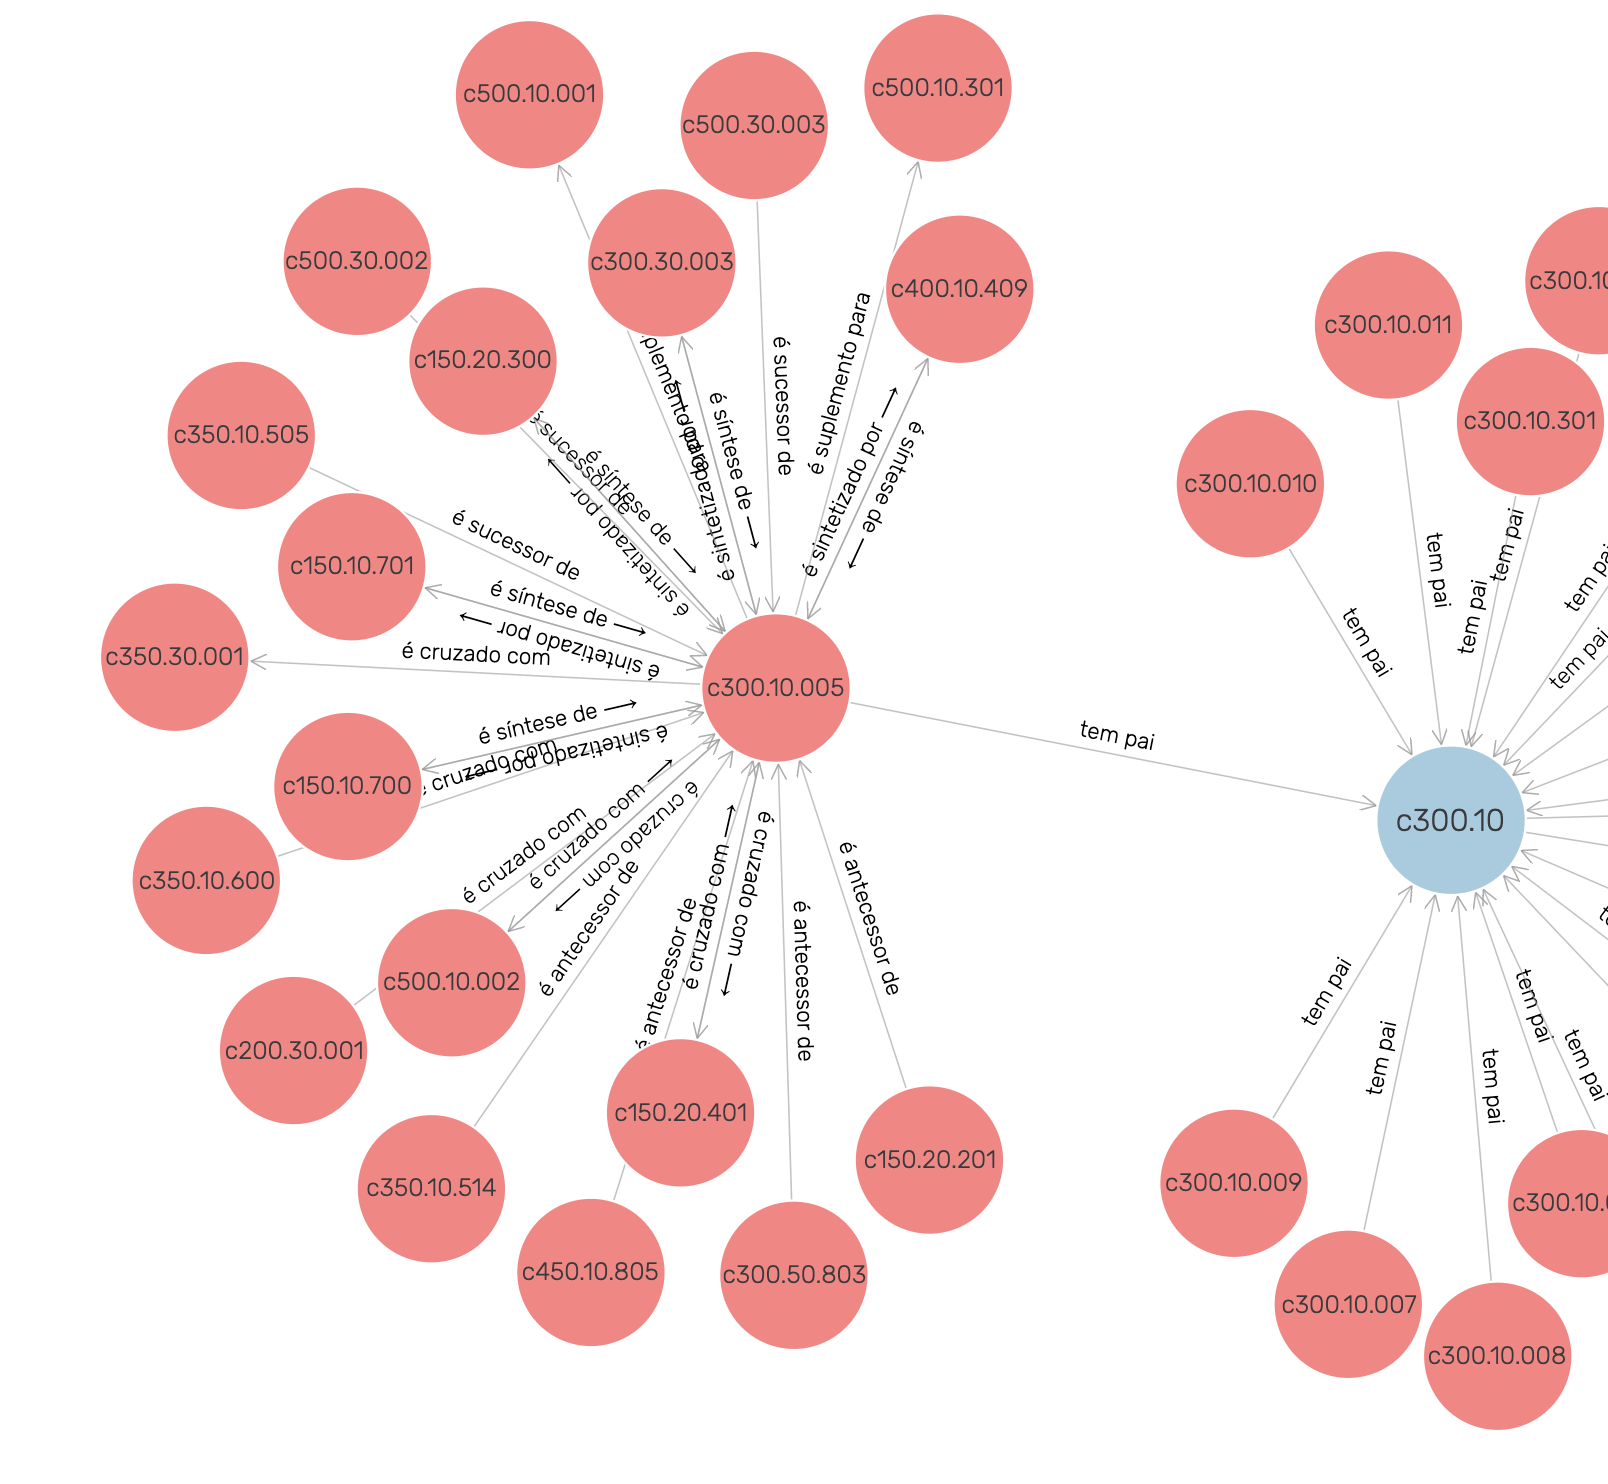
\includegraphics[width=5cm]{./onto.png}\\
\end{flushleft}
\end{minipage}

&

\begin{minipage}{0.4\textwidth}

\vspace{2cm}

 \begin{flushleft}
 
\textsc{\LARGE 
\textbf{Relatório Técnico}
}\\[1.5cm]
 
\large Requisitos de uma plataforma que auxilie na produção de atos normativos
\vspace{3cm}
\end{flushleft}
\end{minipage}

\\
\end{tabular*}

\normalsize
\begin{center}
    \begin{tabular}{l|r}
        ID Documento      & RT-\dataansi-\destsigla \\\hline
        Versão                   & 1.0 \\\hline
        Acesso                  & Restrito \\\hline
        Data de emissão & \data \\\hline
        Autor                      & José Carlos Ramalho \\\hline
        Colaborador & Luís Filipe Cunha \\\hline
        Destinatário         & \destinatario\\\hline                         
    \end{tabular}
\end{center}

 
\end{titlepage}


\tableofcontents

\chapter{Entidade Executante}

O Departamento de Informática da Universidade do Minho (DIUM) tem por missão a divulgação do conhecimento, 
fundamental e especializado, nas áreas da ciência e das tecnologias da computação, com particular destaque para a 
Programação associada à Verificação e Segurança, os Sistemas Inteligentes, os Sistemas Distribuídos e confiáveis, 
os Sistemas de Computação de Alto-desempenho, a Engenharia de Software e as Comunicações e Redes de Computadores.

Aposta numa abordagem rigorosa à resolução de problemas por computador com base na adopção de modelos formais e 
métodos sistemáticos de análise e desenvolvimento. Cumpre a sua missão:

\begin{itemize}
    \item Lecionando cursos de licenciatura, e pós-graduação: mestrado e doutoramento;
    \item Realizando projetos de investigação e desenvolvimento internos e externos à Universidade.
\end{itemize}

Conta para isso com um pessoal permanente de cerca de 52 Docentes (todos doutorados) e 10 técnicos e mais de uma dezena 
de professores convidados para reforço das várias equipes docentes. Aos cursos que oferece, assegura um nível de ensino 
de qualidade elevada, demonstrada quer pelo avultado número de candidatos às suas ofertas formativas, quer pela grande e 
continuada procura dos estudantes formados pelo DIUM por parte dos empregadores nacionais e estrangeiros.

Para criar e manter actual o conhecimento que ensina e aplica, a actividade de investigação dos seus docentes está enquadrada 
em vários centros de investigação. Aqui exploram a teoria e desenvolvem projetos de concretização, com a colaboração de bolseiros 
de vários níveis (desde iniciação à investigação a pós-doutorados), Associação de Estudantesde pós-graduação e de pós-doutoramento.


\section{Informação de Contacto}

\begin{center}
\begin{tabular}{l|r}
Endereço Web                 & \url{http://www.di.uminho.pt} \\\hline
Telefone                            & +351 253 604430 \\\hline
Correio electrónico          & jcr@di.uminho.pt \\\hline
Responsável do projeto       & José Carlos Ramalho \\\hline
Morada                       & Departamento de Informática\\
                             & Universidade do Minho\\
                             & 4710-057 Gualtar, Braga\\\hline                         
\end{tabular}
\end{center}
\chapter{Sumário executivo}

Este documento descreve os trabalhos realizados no âmbito do levantamento de requisitos para o desenvolvimento 
de uma plataforma que deverá auxiliar na produção de atos normativos.

Este trabalho desenvolve-se no âmbito do procedimento com a Ref.ª PRR-12257-23-04 materializado num contrato 
entre a Direção Geral de Política da Justiça (DGPJ) e a Universidade do Minho (UM).

Um ato normativo é materializado num documento legislativo.
Há várias tipologias de documentos legislativos, várias dezenas.
Tratá-las todas está fora do âmbito deste projeto.
A entidade adjudicante designou como prioritárias o decreto-regulamentar, o decreto, a portaria e o despacho normativo 
(publicado na 2.a série do Diário da República) e, em certos casos, a resolução do Conselho de Ministros.

Ao longo do documento, iremos descrever as etapas do desenvolvimento do 
projeto identificando, para cada uma,
os requisitos que se vão identificando e a forma de os cumprir.

No fim, em anexo, apresenta-se uma porposta de caderno de encargos para o 
desenvolvimento da plataforma.

\chapter{Introdução}

Esta atividade tem por objetivo a definição dos requisitos de uma plataforma
que auxilie na produção de atos normativos, com recurso a mecanismos de 
Inteligência Artificial (IA), em concordância
com os elementos apurados na atividade anterior do estudo 
(as melhores práticas existentes nos
sistemas de informação utilizados para apoio à redação legislativa), 
que suportem os requisitos técnicos do procedimento a lançar para a execução 
da plataforma e que deve cumprir com as caraterísticas que se descrevem nas secções seguintes.

\section{Tipologias de atos normativos}

Como já foi referido no resumo, houve necessidade de limitar as tipologias de atos normativos.
A entidade adjudicante designou como prioritárias o decreto-regulamentar, o decreto, a portaria e o despacho normativo 
(publicado na 2.a série do Diário da República) e, em certos casos, a resolução do Conselho de Ministros.

No capítulo \ref{tipologias}, apresenta-se uma análise realizada pela equipa de Direito da UM, onde se pretendeu perceber 
qual a estrutura de cada tipologia e quais os campos de metadados mais relevantes em cada uma.

\section{Requisitos}

Foram definidos, à partida, vários requisitos que se agruparam nas seguintes categorias:

\begin{itemize}
\item Requisitos funcionais de alto nível
\item Requisitos funcionais
\item Requisitos de interoperabilidade
\item Identificação dos mecanismos de IA e das ferramentas conexas a usar no desenvolvimento
da plataforma
\item Requisitos da infraestrutura
\end{itemize}

No capítulo \ref{requisitos}, faz-se uma análise detalhada de cada um.


\section{Protótipo/Prova de Conceito}

Além dos relatórios produzidos, será desenvolvida uma prova de conceito, a uma escala
reduzida, que permitirá elucidar alguns dos requisitos e, provavelmente, levantar novos requisitos ainda
não especificados.

A prova de conceito a desenvolver será composta pelas seguintes atividades e respetivos
resultados:

\begin{itemize}
\item Adoção do software open source LEOS (Legislation Editing Open Software ), como base da
solução, instalação e disponibilização online;
\item Colheita de um subconjunto de legislação do DRE;
\item Colheita de algumas bases de dados de jurisprudência dos tribunais;
\item Especificação de um modelo ontológico para a legislação colhida (baseada no trabalho já
realizado pelo EPO no ELI);
\item Processamento/Mineração, usando técnicas de NLP (Natural Language Processing ), da
legislação colhida para extração de dados para o povoamento da ontologia especificada;
\item Disponibilização da ontologia através de um motor de gestão de bases de dados orientadas a
grafos online;
\item Disponibilização de uma interface de pesquisa baseada em SPARQL que permitirá navegar na
ontologia;
\item Integração do LEOS com a base de dados ontológica: como suporte à edição de legislação;
\item  (Possibilidade) Identificar os vários tipos de documentos legislativos e estudar a hipótese de
aplicar técnicas de Machine Learning (ML) para gerar automaticamente conteúdo novo no
documento que está a ser editado.
\end{itemize}

No capítulo \ref{prototipo}, apresenta-se o trabalho realizado que conduziu à versão do protótipo em linha.


\chapter{Tipologias de atos normativos}
\label{tipologias}

A plataforma que se pretende criar deverá ter modelos pré-criados para todas as tipologias de atos normativos 
que se venham a suportar. 
Um modelo de uma tipologia pressupõe a especificação estrutural dos documentos pertencentes a essa tipologia, 
podendo também conter uma sugestão de texto a incluir nos vários elementos estruturais que a compoem.

No contexto legístico português há dezenas de tipologias. No âmbito deste trabalho e devido a 
restrições temporais, foi necessário reduzir a um subconjunto mas significativo e representativo do que se pretende.

Consultou-se a entidade adjudicante que designou como prioritárias a lei, o decreto-regulamentar, o decreto, 
a portaria e o despacho normativo 
(publicado na 2.a série do Diário da República) e, em certos casos, a resolução do Conselho de Ministros.

\section{Metadados}

Depois de uma análise feita sobre vários documentos de cada uma destas tipologias, chegou-se ao seguinte conjunto
de metadados, comuns a todas:

\begin{description}
    \item[referencia] - fórmula usualmente utilizada para identificar os diplomas; 
    Normalmente, os documentos dentro de uma tipologia 
    são referenciados por combinação de tipologia, número de série e ano;
    \item[tipologia] - designação da tipologia: \texttt{Lei}, \texttt{Decreto-lei}, etc;
    \item[localPublicacao] - local de publicação, 1.ª ou 2.ª Série do 
    Diário da República;
    \item[numPublicacao] - número de publicação, número atribuído sequencialmente 
    dentro do mesmo ano e da mesma tipologia;
    \item[dataPublicacao] - data de publicação do diploma;
    \item[emissor] - entidade emissora; Pode ser a Assembleia da República, o Governo, 
    a Presidência do Conselho de Ministros, um Ministério em Especial ou uma Secretaria 
    de Estado de algum Ministério;
    \item[sumario] - contém a indicação do assunto principal do diploma;
    \item[preambulo] - contém um enquadramento legal e justificativo do diploma, 
    que normalmente termina com a indicação de que a entidade emissora \emph{"decreta o seguinte"};
    \item[articulado] - contém a parte dispositiva do diploma, artigos/normas legais;
    \item[anexos] - pode conter ou não; são usualmente colocadas as tabelas, listagem, mapas, símbolos, 
    ou outros elementos gráficos ou quantitativos referidos no articulado.
\end{description}

No seguimento desta análise, referem-se exemplos reais de documentos nas tipologias selecionadas e apresentam-se 
exemplos de como seriam os respetivos registos de metadados em XML. Escolhe-se o XML por ser um formato aberto,
e por ser o formato a usar na plataforma a ser desenvolvida.

\section{Lei}

Um documento desta tipologia pode ser definido como um ato legislativo, emanado pela Assembleia da República, 
no exercício da sua função legislativa, ao abrigo do artigo 164.º e 165.º da Constituição da República Portuguesa.

As leis da Assembleia da República obedecem ao formulário seguinte:
\begin{quoting}
A Assembleia da República decreta, nos termos da alínea... do artigo 161.º da Constituição, o seguinte:
(Segue-se o texto)
\end{quoting}

Tratando-se de lei constitucional ou orgânica, deve mencionar-se expressamente o termo correspondente, 
na parte final da fórmula. 

Tratando-se de resoluções de aprovação de tratados ou acordos internacionais, o texto é composto do seguinte modo:
\begin{quoting}
Aprovar (para ratificação, no caso dos tratados) o ... 
(segue-se a identificação do tratado ou do acordo internacional em forma simplificada, 
com indicação da matéria a que respeita, do local e data da assinatura, sendo o teor do respetivo 
instrumento publicado em anexo).
\end{quoting}

\subsection{Exemplo: Lei n.º 74/98, de 11 de novembro} 

O seu registo de metadados teria a seguinte extrutura em XML:

\begin{Verbatim}[frame=single, numbers=left, fontsize=\small, commandchars=\\\{\}]
<?xml version="1.0" encoding="UTF-8"?>
<documento>
    <referencia>Lei 74/98</referencia>
    <tipologia>Lei</tipologia>
    <localPublicacao>1.ª Série</localPublicacao>
    <numPublicacao>74</numPublicacao>
    <dataPublicacao>1998-11-11</dataPublicacao>
    <emissor>Assembleia da República</emissor>
    <sumario>Publicação, identificação e formulário 
            dos diplomas.</sumario>
    <preambulo>A Assembleia da República decreta, 
            nos termos da alínea c) do artigo 161.º da 
            Constituição, para valer como lei geral da República, 
            o seguinte:</preambulo>
    <articulado>ver diploma</articulado>
    <anexos>ver diploma</anexos>
</documento>
\end{Verbatim}


\section{Decreto-lei}

Um documento desta tipologia pode ser definido como um ato legislativo, diploma do Governo, no exercício 
da sua função legislativa, ao abrigo do artigo 198.º da Constituição da República Portuguesa.

Os decretos-lei têm o seguinte formulário:

\begin{description}
    \item[Decretos-leis previstos na alínea a) do n.º 1 do artigo 198.º da Constituição]: 
    
    \begin{quoting}
        Nos termos da alínea a) do n.º 1 do artigo 198.º da Constituição, o Governo decreta o seguinte:
        (Segue-se o texto.)
    \end{quoting}

    \item[Decretos-leis previstos na alínea b) do n.º 1 do artigo 198.º da Constituição]: 
    
    \begin{quoting}
        No uso da autorização legislativa concedida pelo artigo... da Lei n.º ...., de... 
        de..., e nos termos da alínea b) do n.º 1 do artigo 198.º da Constituição, 
        o Governo decreta o seguinte:
        (Segue-se o texto.)
    \end{quoting}

    \item[Decretos-leis previstos na alínea c) do n.º 1 do artigo 198.º da Constituição]: 
    
    \begin{quoting}
        No desenvolvimento do regime jurídico estabelecido pela Lei (ou Decreto-Lei) n.º ...., 
        de... de..., e nos termos da alínea c) do n.º 1 do artigo 198.º da Constituição, 
        o Governo decreta o seguinte:
        (Segue-se o texto.)
    \end{quoting}

    \item[Decretos-leis previstos no n.º 2 do artigo 198.º da Constituição]: 
    
    \begin{quoting}
        Nos termos do disposto no n.º 2 do artigo 198.º da Constituição, o Governo decreta o seguinte:
        (Segue-se o texto.)
    \end{quoting}

\end{description}

\subsection{Exemplo: DL n.º 4/2024, de 5 de janeiro} 
    
O seu registo de metadados teria a seguinte extrutura em XML:
    
\begin{Verbatim}[frame=single, numbers=left, fontsize=\small, commandchars=\\\{\}]
<?xml version="1.0" encoding="UTF-8"?>
    <documento>
        <referencia>DL 4/2024</referencia>
        <tipologia>DL</tipologia>
        <localPublicacao>1.ª Série</localPublicacao>
        <numPublicacao>4</numPublicacao>
        <dataPublicacao>2024-01-05</dataPublicacao>
        <emissor>Presidência do Conselho de Ministros</emissor>
        <sumario>Institui o mercado voluntário de carbono e 
            estabelece as regras para o seu funcionamento.</sumario>
        <preambulo>ver diploma</preambulo>
        <articulado>ver diploma</articulado>
        <anexos>ver diploma</anexos>
    </documento>
\end{Verbatim}


\section{Decreto}

Um documento desta tipologia pode ser definido como um Diploma do Governo que visa aprovar 
os acordos internacionais, ao abrigo do artigo 197.º, n.º 1, al. c), da Constituição da 
República Portuguesa.

Os decretos têm o seguinte formulário:

\begin{quoting}
    Nos termos da alínea c) do n.º 1 do artigo 197.º da Constituição, o Governo aprova 
    o... (segue-se a identificação do acordo internacional em forma simplificada, com 
    indicação da matéria a que respeita, do local e da data da assinatura, sendo o 
    teor do respetivo instrumento publicado em anexo).
\end{quoting}


\subsection{Exemplo: Decreto 1/2024, de 22 de janeiro} 
    
O seu registo de metadados teria a seguinte extrutura em XML:
    
\begin{Verbatim}[frame=single, numbers=left, fontsize=\small, commandchars=\\\{\}]
<?xml version="1.0" encoding="UTF-8"?>
    <documento>
        <referencia>Decreto 1/2024</referencia>
        <tipologia>Decreto</tipologia>
        <localPublicacao>1.ª Série</localPublicacao>
        <numPublicacao>1</numPublicacao>
        <dataPublicacao>2024-01-22</dataPublicacao>
        <emissor>Presidência do Conselho de Ministros</emissor>
        <sumario>Aprova o Acordo de Cooperação Económica entre a 
            República Portuguesa e a República da Moldova.</sumario>
        <preambulo>ver diploma</preambulo>
        <articulado>ver diploma</articulado>
        <anexos>ver diploma</anexos>
    </documento>
\end{Verbatim}


\section{Decreto-Regulamentar}

Um documento desta tipologia pode ser definido como um Regulamento. É um diploma do Governo, 
no exercício da sua função administrativa, ao abrigo dos artigos 199.º, als. c) ou g), e 
112.º, n.º 6 . É pouco comum.

Os decretos-regulamentares têm o seguinte formulário:

\begin{quoting}
    Nos termos da alínea c) do artigo 199.º da Constituição e... 
    (segue-se a identificação do ato legislativo a regulamentar), 
    o Governo decreta o seguinte: : 
    (segue-se o texto)
\end{quoting}


\subsection{Exemplo: DR 3/2024, de 21 de fevereiro} 
    
O seu registo de metadados teria a seguinte extrutura em XML:
    
\begin{Verbatim}[frame=single, numbers=left, fontsize=\small, commandchars=\\\{\}]
<?xml version="1.0" encoding="UTF-8"?>
    <documento>
        <referencia>DR 3/2024</referencia>
        <tipologia>Decreto-Regulamentar</tipologia>
        <localPublicacao>1.ª Série</localPublicacao>
        <numPublicacao>3</numPublicacao>
        <dataPublicacao>2024-02-21</dataPublicacao>
        <emissor>Presidência do Conselho de Ministros</emissor>
        <sumario>Procede à fixação do universo dos contribuintes 
            abrangidos pela declaração automática de rendimentos.
        </sumario>
        <preambulo>ver diploma</preambulo>
        <articulado>ver diploma</articulado>
        <anexos>ver diploma</anexos>
    </documento>
\end{Verbatim}


\section{Resolução do Conselho de Ministros}

Um documento desta tipologia pode ser definido como uma resolução emanada quando 
o Governo reúne em plenário, concretiza-se o Conselho de Ministros. 
É um ato normativo do Governo no exercício da sua função administrativa.

As Resoluções do Conselho de Ministros têm o seguinte formulário:

\begin{quoting}
    Nos termos da alínea... do artigo 199.º da Constituição, o Conselho de Ministros 
    resolve:
        (Segue-se o texto.)
\end{quoting}

Ou:
\begin{quoting}
    Nos termos do... (segue-se a identificação do ato e da respetiva norma que 
    estabelece a exigência de resolução) e da alínea... do artigo 199.º da Constituição, 
    o Conselho de Ministros resolve:
    (Segue-se o texto.)
\end{quoting}


\subsection{Exemplo: RCM 28/2024, de 23 de fevereiro} 
    
O seu registo de metadados teria a seguinte extrutura em XML:
    
\begin{Verbatim}[frame=single, numbers=left, fontsize=\small, commandchars=\\\{\}]
<?xml version="1.0" encoding="UTF-8"?>
    <documento>
        <referencia>RCM 28/2024</referencia>
        <tipologia>RCM</tipologia>
        <localPublicacao>1.ª Série</localPublicacao>
        <numPublicacao>28</numPublicacao>
        <dataPublicacao>2024-02-23</dataPublicacao>
        <emissor>Presidência do Conselho de Ministros</emissor>
        <preambulo>ver diploma</preambulo>
        <articulado>ver diploma</articulado>
        <anexos>ver diploma</anexos>
    </documento>
\end{Verbatim}

O campo \texttt{sumário} considera-se não aplicável nesta tipologia.


\section{Portaria}

Um documento desta tipologia pode ser definido como um diploma do Governo, 
no exercício da sua função administrativa. 
É muito comum que a própria lei determine a sua execução mediante portaria.

As Portarias têm o seguinte formulário:

\begin{quoting}
    Manda o Governo, pelo... (indicar o membro ou membros competentes), 
    o seguinte: 
    (Segue texto)
\end{quoting}


\subsection{Exemplo: Portaria 68/2024, de 23 de Fevereiro} 
    
O seu registo de metadados teria a seguinte extrutura em XML:
    
\begin{Verbatim}[frame=single, numbers=left, fontsize=\small, commandchars=\\\{\}]
<?xml version="1.0" encoding="UTF-8"?>
    <documento>
        <referencia>Portaria 68/2024</referencia>
        <tipologia>Portaria</tipologia>
        <localPublicacao>1.ª Série</localPublicacao>
        <numPublicacao>68</numPublicacao>
        <dataPublicacao>2024-02-23</dataPublicacao>
        <emissor>Presidência do Conselho de Ministros</emissor>
        <sumario>Décima segunda alteração ao Regulamento Específico 
            do Domínio da Competitividade e Internacionalização
        </sumario>
        <preambulo>ver diploma</preambulo>
        <articulado>ver diploma</articulado>
        <anexos>ver diploma</anexos>
    </documento>
\end{Verbatim}


\section{Despacho Normativo}

Um documento desta tipologia pode ser definido como um diploma do Governo, 
no exercício da sua função administrativa. 

Os Despachos Normativos têm o seguinte formulário:

\begin{quoting}
    (Inicia por identificar o acto legislativo que lhe serve de base.)
\end{quoting}


\subsection{Exemplo: DN 1/2024, de 5 de janeiro} 
    
O seu registo de metadados teria a seguinte extrutura em XML:
    
\begin{Verbatim}[frame=single, numbers=left, fontsize=\small, commandchars=\\\{\}]
<?xml version="1.0" encoding="UTF-8"?>
    <documento>
        <referencia>DN 1/2024</referencia>
        <tipologia>DN</tipologia>
        <localPublicacao>2.ª Série</localPublicacao>
        <numPublicacao>1</numPublicacao>
        <dataPublicacao>2024-01-05</dataPublicacao>
        <emissor>Gabinete do Secretário de Estado do Turismo, 
            Comércio e Serviços (Ministério da Economia e Mar)
        </emissor>
        <sumario>Prorroga o prazo de apresentação de candidaturas ao 
            concurso específico da Linha Interior + Turismo, aberto 
            na sequência dos incêndios de 4 e 5 de agosto de 2023
        </sumario>
        <preambulo>ver diploma</preambulo>
        <articulado>ver diploma</articulado>
        <anexos>ver diploma</anexos>
    </documento>
\end{Verbatim}

\section{Sumário}

Ao longo deste capítulo, foram caraterizadas as tipologias de atos normativos que serão 
consideradas neste trabalho conducente a uma prova de conceito.

Já existe um formato aberto definido para o intercâmbio deste tipo de informação a nível europeu.
Esse formato está especificado num XML Schema, por isso se adiantou com uma possível
instância XML para cada um dos tipos de registo.



\chapter{Requisitos}
\label{requisitos}

Na proposta subjacente ao contrato ao abrigo do qual se redige este relatório, constavam vários grupos de requisitos.
Neste capítulo, contextualiza-se cada um deles de acordo com o protótipo (cap. \ref{prototipo}) instalado, parametrizado 
e desenvolvido.

Relativamente ao protótipo, era um requisito que este se baseasse na plataforma LEOS (\emph{"Legislation Editing Open Software"}).
O LEOS tem já desenvolvidos e implementados muitos dos requisitos, carecendo de uma adaptação à realidade portuguesa.
Ao longo deste capítulo, faz-se uma associação de cada um dos requisitos a uma ou mais funcionalidades da plataforma LEOS,
indicando as parametrizações que será necessário fazer. Para os casos em que a associação não seja possível indicam-se as 
funcionalidades a desenvolver.

A criação desta nova plataforma pressupõe também uma ligação automática (iteroperabilidade) a outro sistema onde estaria 
a jurisprudência nacional. Para isso, seria necessário que existisse uma normalização sobre a jurisprudência e que esta fosse 
disponibilizada numa API de dados. Algo que poderá acontecer num futuro próximo.

\section{Requisitos}

Nas subsecções seguintes descrevem-se os conceitos associados a cada requisito, se estão ou não presentes no LEOS e,
o que será preciso fazer caos não estejam.

\subsection{Requisitos funcionais}

Alguns destes requisitos estão relacionados com políticas sobre a adoção de normas e a especificação e 
criação de processos, no entanto,
ao colocarmos o LEOS como base, algumas destas decisões já foram tomadas e parte deste trabalho já está feita.

\subsubsection{Deteção automática de cumprimento de normas de produção de atos normativos}

O LEOS precisa de ser parametrizado com os modelos estruturais dos atos normativos que se pretendem criar.
No capítulo anterior, apresentou-se uma análise prévia necessária à criação destes modelos. 
O passo seguinte, será 
especificar esses modelos em XML numa linguagem específica desenvolvida para o efeito (\cite{akoma-ntoso}).
Apresentam-se exemplos mais à frente \ref{???}.

Esta especificação de cada um dos modelos pode e deve incluir os requisitos estruturais que devem ser observados na 
produção de atos normativos. Ao fazê-lo, o LEOS ou outra plataforma que os venha a utilizar pode verificar automaticamente 
o cumprimento dos requisitos/normas.

\subsubsection{Observação de interpretações firmadas em jurisprudência sobre normas}

Pedir esclarecimentos.

\subsubsection{Apoio à elaboração de tarefas de avaliação normativa}

Pedir esclarecimentos.

\subsubsection{Automatização dos processos de avaliação legislativa para textos preparados na plataforma}

Pedir esclarecimentos.

\subsubsection{Verificação e validação das referências normativas e legais identificadas nos textos preparados
na plataforma (verificação da existência das normas invocadas)}



\subsubsection{Pesquisa e identificação automática de legislação e jurisprudência}

\subsubsection{Verificação semântica das normas invocadas}

\subsubsection{Descrição dos workflows para a criação e gestão de atos normativos}

(Possibilidade) Descrição destes processos em BPMN

(Possibilidade) Descrição do ciclo de vida dos documentos na plataforma.


\subsection{Requisitos de interoperabilidade}

Hoje em dia, falar de interoperabilidade é quase um requisito mas muitos desconhecem que esta é complexa 
e pode ser considerada em vários e diferentes níveis.

Da bibliografia, interoperabilidade é a capacidade de um sistema (informatizado ou não) de comunicar de 
forma transparente (ou o mais próximo disso) com outro sistema (semelhante ou não).

A nossa Administração Pública (AP) definiu um modelo para a interoperabilidade:
\begin{itemize}
\item Neste contexto, a interoperabilidade consiste na capacidade das organizações interagirem 
e agirem em prol de benefícios comuns, através de comunicação e partilha de informação e conhecimento;
\item O modelo foi baseado na \emph{Framework Europeia de Interoperabilidade}, criada pela Comissão Europeia;
\item Está organizado em quatro camadas: legal, organizacional, técnica e semântica.
\end{itemize}

Apesar de independentes, as quatro camadas são interdependentes, sendo que para se conseguir atingir a interoperabilidade 
semântica, as outras terão de estar contempladas (neste projeto é importante atingir o patamar semântico).


\begin{itemize}
\item Integração com fontes primárias fundamentais, designadamente bases de dados, com toda a
legislação e atos normativos, para apoio à redação legislativa e normativa: p.e., Diário da
República;
\item Integração com fontes primárias de jurisprudência: p. ex., ECLI;
\item Integração com entidades parceiras identificadas para o fornecimento de dados;
\item Interoperabilidade técnica: protocolos de comunicação, API de dados REST ou Web Service ;
\item Interoperabilidade Sintática: formato de importação e exportação de dados; deverá ser baseado
em XML e seguir normas internacionais (Akoma Ntoso XML format, uma norma OASIS para
documentos legislativos);
\item Interoperabilidade Semântica: representação semântica dos dados, ontologias OWL, utilização
do ELI e da ontologia associada;
\end{itemize}

\subsection{Identificação dos mecanismos de IA e das ferramentas conexas a usar no desenvolvimento
da plataforma}

\begin{itemize}
\item Utilização de mecanismos de Processamento de Linguagem Natural (PLN) e Mineração de
Texto, para extração de representação e significados dos textos disponíveis na base de dados
da plataforma;
\item Utilização de aprendizagem pela máquina (Machine Learning ) para incrementar a precisão do
sistema (processo de validação pelo utilizador/Configurador);
\item Definição de regras de mapeamento para aumentar a precisão das árvores de decisão
adotadas;
\item Definição de estratégia de redes neuronais para efeitos de utilização de sistemas de previsão,
designadamente na identificação de legislação e jurisprudência;
\item Identificação dos algoritmos mais adequados e o seu futuro desenvolvimento;
\item Identificação das necessidades de treino do sistema de IA.
\end{itemize}


\subsection{Requisitos da infraestrutura}

\begin{itemize}
\item Arquitetura global da plataforma;
\item Identificação dos serviços que devem compor o sistema;
\item Identificação dos requisitos técnicos de cada serviço;
\item Identificação/previsão das necessidades de processamento, espaço de armazenamento e
conectividade;
\item A Identificação de necessidade de computação em Cloud ou on-premises e respetivos
requisitos;
\item Identificação dos requisitos de interoperabilidade face a sistemas externos (comunicação,
armazenamento e representação dos dados): por exemplo, bases de dados do DRE - INCM e
de Jurisprudência dos tribunais, Ministério da Justiça (MJ), IGFEJ, 
Conselho Superior da Magistratura (CSM).
\end{itemize}


\subsection{Requisitos de sustentabilidade}





\chapter{Protótipo/Prova de Conceito}
\label{prototipo}

Neste capítulo, descrevem-se os trabalhos conducentes à criação da prova de conceito do sistema a desenvolver. 
Começa-se com uma pequena introdução contextual para logo entrar nos detalhes técnicos.

\section{Introdução}

Além dos relatórios produzidos, será desenvolvida uma prova de conceito, a uma escala
reduzida, que permitirá elucidar alguns dos requisitos e, provavelmente, levantar novos requisitos ainda
não especificados.

A prova de conceito a desenvolver será composta pelas seguintes atividades e respetivos
resultados:

\begin{itemize}
\item Adoção do software open source LEOS (Legislation Editing Open Software ), como base da
solução, instalação e disponibilização online;
\item Colheita de um subconjunto de legislação do DRE;
\item Colheita de algumas bases de dados de jurisprudência dos tribunais;
\item Especificação de um modelo ontológico para a legislação colhida (baseada no trabalho já
realizado pelo EPO no ELI);
\item Processamento/Mineração, usando técnicas de NLP (Natural Language Processing ), da
legislação colhida para extração de dados para o povoamento da ontologia especificada;
\item Disponibilização da ontologia através de um motor de gestão de bases de dados orientadas a
grafos online;
\item Disponibilização de uma interface de pesquisa baseada em SPARQL que permitirá navegar na
ontologia;
\item Integração do LEOS com a base de dados ontológica: como suporte à edição de legislação;
\item  (Possibilidade) Identificar os vários tipos de documentos legislativos e estudar a hipótese de
aplicar técnicas de Machine Learning (ML) para gerar automaticamente conteúdo novo no
documento que está a ser editado.
\end{itemize}

\section{LEOS: Legislation Editing Open Software}

O LEOS é um projeto no âmbito da iniciativa \emph{"Interoperable Europe"} da Comissão Europeia para uma política reforçada de 
interoperabilidade do setor público, financiado pelo Programa Digital \emph{Europe (DIGITAL)} e criado para atender à 
necessidade da administração pública e das Instituições Europeias de gerar projetos de legislação em formato XML jurídico.

O projeto LEOS concentra-se em apoiar o co-desenvolvimento, co-design e co-implementação de um "ecossistema de Tecnologias de 
Informação (TI) centrado num LEOS aumentado".

O LEOS foi criado para abordar a modernização e transformação digital da elaboração e revisão de legislação nas 
Instituições da UE, agências e órgãos da UE e Estados-Membros.

Esta plataforma garante que o conteúdo elaborado pelos utilizadores siga as diretrizes de redação, oferecendo recursos como a
aplicação de estruturas de documento pré-definidas, layout pré-definido e regras de numeração. 
Tudo isso para garantir que o autor se possa focar na elaboração do texto e muito menos na gestão do layout (ou verificação). 
Para facilitar a colaboração online eficiente, o LEOS também possui outros recursos como comentários, sugestões, 
controle de versão, edição colaborativa, etc.


\section{Stack Tecnológica}

O LEOS é um ecossitema de serviços relativamente complexo que se passa a descrever.

\subsection{Frontend: interface com o utilizador}

O frontend da plataforma LEOS foi construído usando a framework Vaadin 8 e o AngularJS. 

O Vaadin \footnote{\url{https://vaadin.com/vaadin-8}} é uma framework Java usada para a criação de interfaces Web. 
Esta framework permite gerar vários componentes UI (\emph{"User Interface"}) usando código em JAVA.
A versão 8 em específico foi descontinuada em 21 de Fevereiro, 2022. 
Esta versão já não recebe suporte por quem a desenvolveu e mantinha.

No desenvolvimento do sistema português é preciso acautelar esta situação.
Confirmar junto da equipa de desenvolvimento do LEOS quais os planos para a substituição deste componente ou, em caso 
da inexistência desses planos prever o seu desenvolvimento numa tecnologia atual.

O AngularJS \footnote{\url{https://angularjs.org/}} é uma framework JavaScript que permite criar interfaces visuais reativas. 
No LEOS utilizou-se esta framework para se desenvolver o cliente de anotações.


\subsection{Backend}

O backend da Plataforma LEOS consiste numa aplicação criada com a framework Spring \footnote{\url{https://spring.io/projects/spring-boot}}. 
Esta framework, desenvolvida em JAVA, é reconhecida pela sua estabilidade e fácil manutenção.

De modo a estabelecer a conexão com a base de dados, a aplicação Spring utiliza o módulo Spring Data JPA \footnote{\url{https://spring.io/projects/spring-data-jpa}}. 
Este módulo cria uma camada de abstração sobre a API de persistência do JAVA (JPA), permitindo armazenar e recuperar 
informação de bases de dados relacionais eficientemente.

Para permitir criar abstrações da base de dados, o LEOS usa o Hibernate.
O Hibernate\footnote{\url{https://hibernate.org/}} é uma framework de \emph{"object-relational mapping"} (ORM) para a linguagem Java. 
Esta framework permite realizar o mapeamento entre os modelos orientados a objetos e as bases de dados relacionais tornando 
transparente para o programador a sua implementação.

Para servir o backend, o LEOS utiliza um servidor web Apache Tomcat para receber e responder aos pedidos HTTP. 
O apache Tomcat é também um Servlet container para aplicações java. 
Na plataforma LEOS, este servidor é responsável por servir a aplicação Spring.

Por último, a framework Mockito\footnote{\url{https://site.mockito.org/}} é utilizada para a realização de testes unitários 
para a linguagem de programação JAVA.

\subsection{Persistência}
 
O LEOS utiliza uma base de dados relacional para guardar toda a informação necessária ao seu funcionamento normal. 
Estas informações incluem dados relacionados com utilizadores, configurações, metadados de documentos, etc. 
Por omissão, é utilizada a base de dados H2\footnote{\url{https://www.h2database.com/html/main.html}} cujas caraterísticas 
principais são ser rápida, fácil de usar, de dimensão pequena, poder ser instanciada num servidor ou em memória e 
poder ser gerida via web.

O LEOS guarda as anotações aos documentos numa base de dados à parte. 
Por omissão, é utilizada uma base de dados H2 em memória.

Além da H2, LEOS utiliza um servidor CMIS\footnote{\url{https://www.oasis-open.org/standard/cmisv1-1/}} 
(\emph{"Content Management Interoperability Services"}) para guardar documentos. 
CMIS é um standard OASIS que permite partilha de informação entre diferentes sistemas de gestão de informação. 
De modo a criar este servidor o LEOS utiliza a  ferramenta OpenCMIS do projeto Apache Chemistry.

\subsection{Sumário}

Concluindo, o LEOS assenta num conjunto de tecnologias diversos, com alguma complexidade e com alguns 
riscos associados identificados em cima: Vaadin 8, AngularJS, JAVA Spring, Spring Data JPA, Hibernate, Apache Tomcat,
Mockito, H2 e CMIS.

\section{Configuração do idioma: português}

O LEOS foi desenvolvido utilizando a norma \texttt{i18n}.

A internacionalização (i18n) é o processo de projetar e desenvolver um produto de software para que possa ser adaptado para 
utilizadores de diferentes culturas e idiomas.

A internacionalização não envolve apenas permitir diferentes idiomas, mas também adaptar o software para aceitar diferentes 
formas de dados e configurações para corresponder aos costumes locais e processá-los corretamente.

O Grupo W3C define a internacionalização como:
\begin{quoting}
A internacionalização é o design e o desenvolvimento de um produto, aplicação ou conteúdo que permite fácil 
adaptação a públicos-alvo de cultura, região ou idioma diferentes.
\end{quoting}



Neste contexto, o LEOS é facilmente adaptável a utilizadores de culturas e línguas diferentes. 

Esta norma garante que os dados associados às traduções da plataforma ficam separados do código principal, 
tornando o processo de adaptação do LEOS para novas línguas flexível e eficiente.

Para se configurar o idioma português para o LEOS foi necessário criar um novo ficheiro JSON com as traduções portuguesas dos 
textos da interface gráfica do LEOS. 

Na pasta \verb|\leos\modules\ui-angular\src\assets\i18n\| já se encontram ficheiros JSON para a lingual Inglesa e Francesa. 
Para gerar a versão Portuguesa, traduziu-se automaticamente todas os textos contidos no ficheiro original em Inglês 
(\texttt{en.json}), 
um processo seguido de revisão manual. 
Desta forma foi criado o ficheiro \texttt{pt.json}, o qual foi depois colocado na mesma pasta que os originais.

De seguida, foi necessário alterar o ficheiro de configuração presente na pasta \\
\verb|\leos\modules\ui-angular\src\config\global.ts|, de modo a incluir o ficheiro com traduções portuguesas no LEOS. 
Esta configuração consistiu em adicionar a string \texttt{"pt"} à lista das \emph{languages}, que faz parte do objeto i18n. 
Foi ainda alterado o atributo \texttt{defaultLanguage} de "en" para "pt", no entanto, esta alteração não demonstrou qualquer 
alteração no comportamento do sistema, dado que o inglês continuou a ser a língua por omissão.

\begin{Verbatim}[frame=single, numbers=left, fontsize=\scriptsize]
i18n: {
    i18nService: {
      defaultLanguage: 'pt',
      languages: ['pt', 'en', 'fr'],
    }, ... 
 },
\end{Verbatim}


\section{Modelos/Templates}

\subsection{Adição de novos modelos}

De momento, a criação de novos modelos para a plataforma LEOS é um processo manual sendo necessário a edição/criação de vários 
ficheiros e a sua colocação em locais estratégicos da plataforma.

Vai-se exemplificar este processo com um caso de estudo simples de uma lei.
Ou seja, assuma-se que se pretende gerar um novo modelo para um ato normativo com a tipologia de Lei.
 
No LEOS, os modelos de atos normativos são representados no formato \texttt{Akoma Ntoso (AKN)} já apresentado anteriromente. 
Desta forma, e para iniciar o processo, é necessário gerar um ficheiro no formato AKN para representar a estrutura de uma Lei. 
De momento o LEOS não fornecesse qualquer ferramenta para gerar este tipo de ficheiros pelo que estes têm de ser gerados 
manualmente.

Depois de gerado, o ficheiro AKN deve ser colocado na pasta dos modelos do LEOS: 
\texttt{\url{LEOS_dir/tools/repositor/server/src/main/resources/leos/templates}}.

Cada modelo associado a um dado ato normativo deve ser acompanhado de um outro ficheiro modelo para gerar a página de capa 
desse ato normativo. Este segundo ficheiro também deve ser colocado na pasta dos modelos.
 
A seguir é necessário adicionar uma nova entrada, para cada modelo, em duas tabelas da base de dados (do LEOS) 
para que o LEOS consiga aceder aos novos modelos.

A título de exemplo, eis as \emph{queries} SQL para um novo modelo:

\begin{Verbatim}[frame=single, numbers=left, fontsize=\scriptsize, commandchars=\\\{\}]
    INSERT INTO CONFIG (NAME,OBJECT_ID,AUDIT_C_BY,AUDIT_C_DATE,
                AUDIT_LAST_M_BY,AUDIT_LAST_M_DATE,LANGUAGE,CATEGORY_ID) 
            VALUES ('LEI-01','0','admin/admin',
                   to_timestamp('22-01-21 08:25:40.328000000',
                   'DD-MM-RR HH24:MI:SSXFF'),'admin/admin',
                   to_timestamp('22-01-21 08:25:40.328000000',
                   'DD-MM-RR HH24:MI:SSXFF'),'PT',
                   (SELECT id from CONFIG_CATEGORIES WHERE 
                     CATEGORY_CODE='TEMPLATE_BILL'));
\end{Verbatim}

e

\begin{Verbatim}[frame=single, numbers=left, fontsize=\scriptsize, commandchars=\\\{\}]
    INSERT INTO CONFIG_VERSION (CONFIG_ID,VERSION_LABEL,VERSION_SERIES_ID,
        VERSION_TYPE,IS_LATEST_MAJOR_VERSION,IS_LATEST_VERSION,
        IS_MAJOR_VERSION,IS_VERSION_SERIES_CHECKED_OUT,AUDIT_C_BY,
        AUDIT_C_DATE,AUDIT_LAST_M_DATE,AUDIT_LAST_M_BY,IS_IMMUTABLE) 
      VALUES ((SELECT id from CONFIG WHERE NAME='LEI-01'),'1.0','1',null,1,1,
        1,0,'admin/admin',to_timestamp('30-03-23 07:38:37.451000000',
        'DD-MM-RR HH24:MI:SSXFF'),to_timestamp('30-03-23 07:38:37.496000000',
        'DD-MM-RR HH24:MI:SSXFF'),'admin/admin',0);
\end{Verbatim}

Para finalizar a configuração, é necessário editar o ficheiro \texttt{catalog.xml}, 
presente na mesma pasta dos modelos, de modo a adicionar os modelos gerados ao catálogo de modelos 
para que estes fiquem disponíveis no LEOS. 
Este ficheiro define a estrutura em árvore apresentada no auxiliar de criação de documentos. 
É aqui que devemos colocar a referência do novo modelo para que ele seja visível na árvore (fig.\ref{fig-catalog}).

\figura{fig-catalog}{./imagens/catalog2.png}{LEOS: árvore de tipologias disponíveis}{width=10cm}
  
Exemplo:
 
\begin{Verbatim}[frame=single, numbers=left, fontsize=\scriptsize, commandchars=\\\{\}]
<?xml version="1.0" encoding="UTF-8" ?>
<catalog lang="PT">
    <item type="CATEGORY" id="c1" enabled="true" key="LAW_INITIATIVE">
        <names>
            <name lang="PT">Atos Normativos</name>
        </names>
        <item type="CATEGORY" id="c1.1" enabled="true" 
              key="ATOS_NORMATIVOS">
            <names>
                <name lang="PT">Lei</name>
                <name lang="EN">Law</name>            </names>
            <item type="TEMPLATE" id="LEI-PR-01;LEI-01" enabled="true" 
                  key="lei-01">
                <names>
                    <name lang="PT">01 - Modelo de Lei</name>
                    <name lang="EN">01 – Law Template</name>
                </names>
                <languages>
                    <language lang="PT">Portuguese</language>
                    <language lang="EN">English</language>
                </languages>
            </item>
        </item>
    </item>
    ... 
</catalog>
\end{Verbatim} 


\section{Interface}

Nesta secção, apresentam-se vários exemplos da interface do LEOS configurada para a realidade portuguesa.

Criaram-se modelos muito simples para as tipologias de atos normativos apenas para efeitos de exemplificação.
 
\figura{fig-catalog}{./imagens/leos_lista02.png}{LEOS: resultados da pesquisa de propostas}{width=15cm}

\figura{fig-catalog}{./imagens/leos_lei.png}{LEOS: modelo de uma lei na plataforma}{width=10cm}

%\input{api}

%\input{autenticacao}

%\input{interface-RADA}

%\input{export}

%\input{conclusao}

\end{document}